\chapter{Information Extraction}

To calculate the similarity between a job and a resume, JobFinder system need the models of them, which are  structured data. To get the structured data, some JRSs ask the job seekers input their profiles in forms field by field, and the recruiter input their job description in the same way as well. However, as we discussed in chapter 2, the users are reluctant to take the tedious process ~\cite{singh2010prospect}. Job seekers prefer upload their resumes directly, and recruiters prefer to post the whole job description to web sites. In this chapter we will explain how the Information Extraction module of the system extracts information from these unstructured data source. 
 
Information Extraction is the task of automatically extracting structured information such as entities, relationships between entities, and attributes describing entities from unstructured sources. ~\cite{sarawagi2008information}.  The IE framework will be introduced below by example of processing the job descriptions.   

\section{Text Processing Pipeline}

The IE module uses five ? six stages in order to extract the information 

In Nature Language Processing, especially in Information Extraction, pipeline is a well adopted architecture~\cite{sarawagi2008information}. The pipeline to process the job descriptions in the system has eight stages, which is shown in Figure~\ref{fig:Pipeline}:

\begin{enumerate}
    \item The HTML parser will parse the web pages of job descriptions, which are obtained from web crawler. The parser will get the HTML element that contains the main content of the job description.
    \item Segment module will separate the job description into paragraphs according to HTML tags at first, then separate each paragraph into sentences.
    \item The sentences will be tokenized into string arrays, and be sent to the classification module. The classification module will determine the category of the sentence, and give the sentence a category mark.
    \item The preprocessing module will delete unreadable characters, and correct some tokens spelling.
    \item The annotation module will annotate the tokens with semantic and ontology labels. After labeling, the sentences will have a multi-layered data structure.
    \item The layered sentences will be matched with pre-defined patterns with the FST library. If any pattern could be matched, the ontology information will be extract and stored in the job model.
    \item After every sentence has be processed with the pipeline, the job model will be created and stored into the database.
\end{enumerate}


\begin{figure}[htbp]
  \centering
  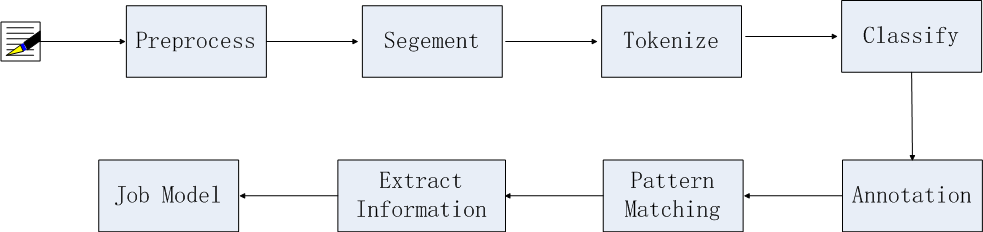
\includegraphics[scale=0.4]{images/pipeline.png}
  \caption{Job Description Process Pipeline}
  \label{fig:Pipeline}
\end{figure}


\section{Machine learning and Rule-based IE technologies}

There are two kinds of competitive techniques in Information Extraction, one is machine learning-based approaches, the other is rule-based approaches. Chiticariu et al. \cite{chiticariu2013rule} summarized the pros and cons of machine learning (ML) and rule-based IE technologies in Table \ref{tab:mlrb}.

\begin{table}[ht]
\caption{Pros and Cons of ML and Rule-Based IE technologies } % title of Table
\centering % used for centering table
\begin{tabular}{ | c |  p{6cm} | p{6cm} | } % centered columns (4 columns)

\hline  %inserts double horizontal lines
 & Pros  & Cons  \\ [0.5ex] % inserts table
%heading
\hline % inserts single horizontal line
Rule-based &
    \begin{singlespace}
       \textbullet~Declarative  \par
       \textbullet~Easy to comprehend\par
       \textbullet~Easy to maintain\par
       \textbullet~Easy to incorporate domain knowledge\par
       \textbullet~Easy to trace and fix the cause of errors  \par
    \end{singlespace}
    &  \begin{singlespace}
      \textbullet~Heuristic \par
       \textbullet~Requires tedious manual labor \par
       \end{singlespace}  \\
\hline
ML-based &
    \begin{singlespace}
       \textbullet~Trainable  \par
       \textbullet~Adaptable \par
       \textbullet~Reduces manual effort \par
    \end{singlespace}
    &  \begin{singlespace}
      \textbullet~Requires labeled data \par
       \textbullet~Requires retraining  for domain adaptation \par
        \textbullet~Requires ML expertise  to use or maintain \par
       \textbullet~Opaque  \par
       \end{singlespace} \\
\hline %inserts single line
\end{tabular}
\label{tab:mlrb} % is used to refer this table in the text
\end{table}

In this work, we prefer the rule-based approach because:
\begin{enumerate}
    \item Most of sentences that contain the information share some common patterns that can be easily identified.
    \item A lot of sentences are not grammatical completed as a sentence, for example some of them missing subject, and some of them are just a list of terms.
    \item Processing speed is also a concern, and generally rule-based approach is faster.
\end{enumerate}


\section{Regular Expression Over Labeled Tokens}

Cascaded Finite-State Transducer is used as a tool to match patterns and extract information for more than 20 years. This approach have been demonstrated very effective in extracting information from text like CIRCUS~\cite{lehnert1991university} and FASTUS~\cite{hobbs199713}.  In the widely used NLP toolkit GATE~\cite{cunningham2002framework}, the semantic tagger JAPE (Java Annotations Pattern Engine) could describe patterns that are used to match and annotate tokens. JAPE adopts a version of CPSL (Common Pattern  Specification Language)~\cite{appelt1998common}, which provides finite state transduction over annotations. Chang et al. presented cascaded regular expressions over tokens~\cite{chang2014tokensregex}, which proposed a cascaded pattern matching tool over token sequences.

After studying these tools, we found most of them are powerful, complex, but not very flexible. One reason is that developers need to learn some DSLs like CPSL, and the other is  integrating the pattern matching tool into the system need extra efforts. So here we proposed a more flexible and lightweight framework, which can do regular expression matching over labeled tokens. The difference between this library and regular expression is that the basic unit to be matched is token, not character. In the library, a pattern is a concatenation of matchers that can match a single token, or a wrapper of other matchers. Currently the library supports seven types of matchers, those are listed in Table~\ref{tab:matchers}.

\begin{table}[ht]
\caption{Matcher Class } % title of Table
\centering % used for centering table
\begin{tabular}{  | l | l | l |  }
 \hline
 Class Name        &  Function                                 & Counter Part of regex    \\
 \hline
 UnitMatcher       &  token is matches the it                  & character  in regex       \\
 \hline
 SequenceMatcher   &  A list of Matcher                        & sequence of characters       \\
  \hline
 QuestionMatcher   &  One or more of the preceding token       & ?       \\
  \hline
 StarMatcher       &  Zero or more of the preceding token      & *       \\
  \hline
 PlusMatcher       &  Zero or one of the preceding token       & +       \\
  \hline
 DotMatcher        &  Any token                                & .      \\
  \hline
 RegexMatcher      &  Any token matches the regular expression               &        \\
  \hline

\end{tabular}
\label{tab:matchers} % is used to refer this table in the text\section{Pipeline of Information Extraction}
\end{table}

The framework supports three styles to create patterns, which gives developers great flexibility. The most common style is defining pattern expression in a string, which is much like traditional regular expression. We give an example as follows:

\begin{framed}
\small
\begin{lstlisting}[language=Python]
seqMatcher =parser.parse("aaa | bbb ccc? * ddd")
\end{lstlisting}
\end{framed}

The seconde style is using algebra operator to connect matchers, as follows:
\begin{framed}
\small
\begin{lstlisting}[language=Python]
Pattern: " aaa (bbb | cccc)"
seqMatcher =  TokenMatcher("aaa") +
    TokenMatcher("bbb") | TokenMatcher("ccc")

\end{lstlisting}
\end{framed}

We also could create complex matcher in programming style, which is like we creating and using some objects when programming, as follows:

\begin{framed}
\small
\begin{lstlisting}[language=Python]
Pattern: " ( aaa | bbb ) cccc "
matcher1 = TokenMatcher("aaa")
matcher2 = TokenMatcher("bbb")
matcher3 = TokenMatcher("ccc")
matcher4 = AlternateMatcher([matcher1,matcher2])
seqMatcher = SeqMatcher([matcher3,matcher4])
\end{lstlisting}
\end{framed}

\section{Implementation of Finite Automata Matching Library }

To transfer a token regular expression to a Finite Automata Transducers(FST), we need two steps: The first is parsing the expression to a tree of matchers, the second is transfer the tree of matchers to the Finite Automata Transducers.

We use PLY(Python Lex-Yacc) as the grammar parser, which  is a pure-Python implementation of the popular compiler construction tools lex and yacc. We defined  grammars of token regular expression in the parser, which can parse the token regular expression to the tree structure.

We use the algorithm proposed by Thompson and Ken\cite{thompson1968programming} to construct the FST from the tree. The state for a regular expression is built up from partial Nondeterministic Finite Automaton (NFA)  for each subexpression, with a different construction for each operator. The partial NFAs have no matching states: instead they have one or more dangling arrows, pointing to nothing. The construction process will finish by connecting these arrows to a matching state.

The NFAs for matching single token is shown in Figure \ref{fig:nfa_single}.

\begin{figure}[htbp]
  \centering
  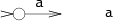
\includegraphics[scale=1]{images/single_token.png}
  \caption{Single Token NFA}
  \label{fig:nfa_single}
\end{figure}

The NFA for the concatenation $e_1e_2$ connects the final arrow of the $e_1$ machine to the start of the $e_2$ machine, which is shown in Figure \ref{fig:nfa_cocat}.

\begin{figure}[htbp]
  \centering
  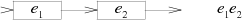
\includegraphics[scale=1]{images/concatenation_tokens.png}
  \caption{Concatenation NFA}
  \label{fig:nfa_cocat}
\end{figure}

The NFA for the alternation $e_1\mid e_2$ adds a new start state with a choice of either the $e_1$ machine or the $e_2$ machine, which is shown in Figure \ref{fig:nfa_alternation}.


\begin{figure}[htbp]
  \centering
  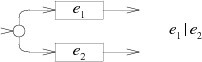
\includegraphics[scale=1]{images/alternation.png}
  \caption{Alternation NFA}
  \label{fig:nfa_alternation}
\end{figure}

The NFA for e? alternates the e machine with an empty path, which is shown in Figure \ref{fig:nfa_question}.


\begin{figure}[htbp]
  \centering
  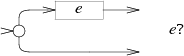
\includegraphics[scale=1]{images/question.png}
  \caption{Zero or one NFA}
  \label{fig:nfa_question}
\end{figure}

The NFA for e* uses the same alternation but loops a matching e machine back to the start, which is shown in Figure \ref{fig:nfa_star}.

\begin{figure}[htbp]
  \centering
  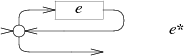
\includegraphics[scale=1]{images/star.png}
  \caption{Zero or more NFA}
  \label{fig:nfa_star}
\end{figure}

The NFA for e+ also creates a loop, but one that requires passing through e at least once, which is shown in Figure \ref{fig:nfa_plus}.

\begin{figure}[htbp]
  \centering
  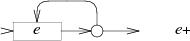
\includegraphics[scale=1]{images/plus.png}
  \caption{One or more NFA}
  \label{fig:nfa_plus}
\end{figure}



The expression like ``DL (, DL])*  (or DL)? DEGREE'' could be transferred to an FST in Figure ~\ref{fig:fst}.

\begin{figure}[htbp]
  \centering
  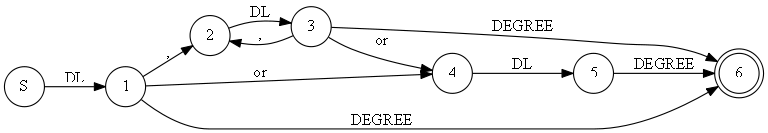
\includegraphics[scale=0.6]{images/test_tokenre2_6.png}
  \caption{Finite Automata Transducers}
  \label{fig:fst}
\end{figure}

\section{Semantic Label}

In the text of natural language, one concept always have some different expressions. For example, the simple concept bachelor's degree,  has several expression in job descriptions, like B.S., BA/BS, 4 years degree, and so on. The Table~\ref{tab:multispelling} shows the words that if followed with word "degree", have the semantic value of ``bachelor's degree''.

\begin{table}[ht]
\caption{All words have meaning bachelors } % title of Table
\centering % used for centering table
\begin{tabular}{  | p{15cm} |  }
 \hline
 "Baccalaureate","bachelors", "bachelor" ,"B.S.", "B.S","BS","BA","BA/BS", "BABS", "BSBA", "B.A." ,"4-year","4-year", "4 year", "four year","college","Undergraduate" , "University" \\
  \hline
\end{tabular}
\label{tab:multispelling} % is used to refer this table in the text\section{Pipeline of Information Extraction}
\end{table}


The regular expression over tokens is a finite state transducer (FST) with states that are the tokens need to be matched with. If all above words are added to the regular expression, the FST will have too many states, and the matching process will be very slow because of the problem of combinatorial explosion.

To resolve this problem, we proposed an approach to use the patterns match the semantic label of the sentences, not the the original text. Because in this system, we don't care what the words the sentences really use, we want to extract the semantic value from the matching phrases.

We transfer the sentences will be matched to a structure with two layers labels. In the first layer, we labeled the word with its semantic value, which is the value that we want to extract from the sentence. In the second layer, the labels are the ontology super class of the first layer labels. For example the word "bachelors" is labeled in the first layer with label "BS LEVEL", which means bachelors degree level, and the word "PhD" is labeled as "PHD LEVEL". In the second layer, they both are labeled with "DEGREE LEVEL", which is the ontology super class of the two labels. A labeled sentence is shown in ~\ref{tab:labeldsent}.

\begin{table}[ht]
\caption{Labeled sentence } % title of Table
\centering % used for centering table
\begin{tabular}{  | c | c | c | c | c |c | c |c | c | c |  }
 \hline
 layer 2 & DE LEVEL   & DEGREE & IN & MAJOR            & OR & MAJOR  &.  \\
 \hline
 layer 1 &  BS LEVEL   & DEGREE & IN & MAJOR CS         & OR & MAJOR INFO & .      \\
 \hline
   words & bachelors   & degree & in & computer science & or & information systems & .     \\
  \hline
\end{tabular}
\label{tab:labeldsent} % is used to refer this table in the text\section{Pipeline of Information Extraction}
\end{table}

We use a dictionary to store the words in sentences and their labels, in which the key is the different spellings an expressions, and the value is the meaning of the concept. For example the Table~\ref{tab:multispelling} shows all keys in the dictionary with and the values ``bachelors''.

After labeling, the sentence become a sequence of arrays, each array includes the original token and its labels in the other two layers. The flexibility of the tool also comes from that developers could determine which layer of the array should be matched, the original text or labels in the first or second layer.  Developers can assign lambda expressions to the matcher's catching function, which defines how to get the matching input,  and out function, which defines what should be outputed. For example, to match the labeled sentence, we set the lambda expression for catching function to ``lambda x:x[2]'', and the out function to ``lambda x:x[1]'', which make the matcher match the label in second layer, and output the the value of semantic value in the first layer. We show some patterns used to match degree phases in Table ~\ref{tab:patterns}.

\begin{table}[ht]
\small
\caption{Patterns match degree} % title of Table
\centering % used for centering table
\begin{tabular}{  | l  |  }
 \hline
 DE\_LEVEL,  DE\_LEVEL, OR  DE\_LEVEL DEGREE   \\
 DE\_LEVEL DEGREE ( IN  $\vert$  OF ) DT MAJOR   \\
 MAJOR\_DEGREE  ,  MAJOR\_DEGREE OR MAJOR \\
 DE\_LEVEL (, DE\_LEVEL)* (OR DE\_LEVEL)? BE? PERFER\_VBD   \\
 \hline
\end{tabular}
\label{tab:patterns} % is used to refer this table in the text\section{Pipeline of Information Extraction}
\end{table}
